%--------------------------------------
%CANEVAS
%--------------------------------------

%utiliser les environnement \begin{comment} \end{comment} pour mettre en commentaire le préambule une fois la programmation appelée dans le document maître (!ne pas oublier de mettre en commentaire \end{document}!)

\begin{comment}

\documentclass[a4paper, 11pt, twoside, fleqn]{memoir}

\usepackage{AOCDTF}

\marqueurchapitre
\decoupagechapitre{1} %juste pour éviter les erreurs lors de la compilation des sous-programmations (passera en commentaire)

%lien d'édition des figures Tikz sur le site mathcha.io (rajouter le lien d'une modification effectuée sur la figure tikz avec le nom du modificateur car il n'y a qu'un lien par compte) 

%lien mathcha Nom Prénom : https://www.mathcha.io/editor/88XmJTWQUxztLv21v6S12z22Lf78mx9yIOvQ9M5

%--------------------------------------
%corps du document
%--------------------------------------

\begin{document} %corps du document
	\openleft %début de chapitre à gauche

\end{comment}

\begin{figure}[h]
\caption{Structure d'un corps d'épreuve}

\tikzset{every picture/.style={line width=0.75pt}} %set default line width to 0.75pt        

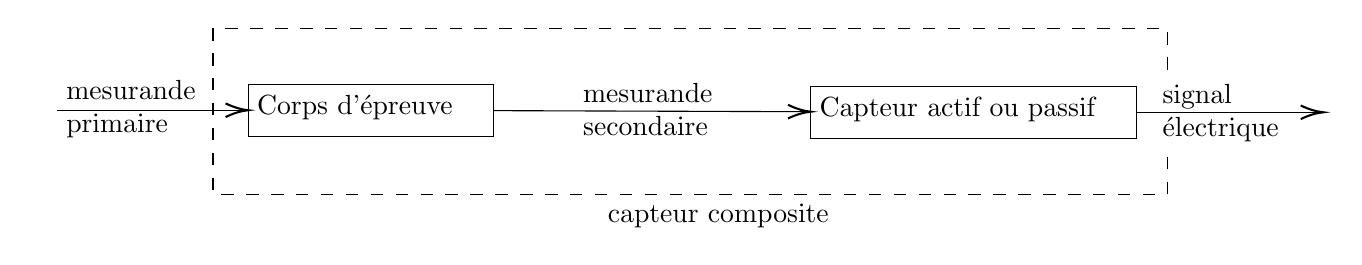
\begin{tikzpicture}[x=0.75pt,y=0.75pt,yscale=-1,xscale=1]
%uncomment if require: \path (0,300); %set diagram left start at 0, and has height of 300

%Straight Lines [id:da6331649314862131] 
\draw  [dash pattern={on 4.5pt off 4.5pt}]  (550,120) -- (550,100) -- (90,100) -- (90,180) -- (550,180) -- (550,160) ;

% Text Node
\draw    (107,127) -- (225,127) -- (225,152) -- (107,152) -- cycle  ;
\draw (110,131) node [anchor=north west][inner sep=0.75pt]   [align=left] {Corps d'épreuve};
% Text Node
\draw    (378,128) -- (535,128) -- (535,153) -- (378,153) -- cycle  ;
\draw (381,132) node [anchor=north west][inner sep=0.75pt]   [align=left] {Capteur actif ou passif};
% Text Node
\draw (1,131) node [anchor=north west][inner sep=0.75pt]   [align=left] {};
% Text Node
\draw (50.5,139) node   [align=left] {mesurande\\primaire};
% Text Node
\draw (299.5,139) node   [align=left] {mesurande\\secondaire};
% Text Node
\draw (628,132) node [anchor=north west][inner sep=0.75pt]   [align=left] {};
% Text Node
\draw (575.5,141) node   [align=left] {signal\\électrique};
% Text Node
\draw (333.5,190.5) node   [align=left] {capteur composite};
% Connection
\draw    (225,139.7) -- (376,140.22) ;
\draw [shift={(378,140.23)}, rotate = 180.2] [color={rgb, 255:red, 0; green, 0; blue, 0 }  ][line width=0.75]    (10.93,-3.29) .. controls (6.95,-1.4) and (3.31,-0.3) .. (0,0) .. controls (3.31,0.3) and (6.95,1.4) .. (10.93,3.29)   ;
% Connection
\draw    (15,139.5) -- (105,139.5) ;
\draw [shift={(107,139.5)}, rotate = 180] [color={rgb, 255:red, 0; green, 0; blue, 0 }  ][line width=0.75]    (10.93,-3.29) .. controls (6.95,-1.4) and (3.31,-0.3) .. (0,0) .. controls (3.31,0.3) and (6.95,1.4) .. (10.93,3.29)   ;
% Connection
\draw    (535,140.5) -- (623,140.5) ;
\draw [shift={(625,140.5)}, rotate = 180] [color={rgb, 255:red, 0; green, 0; blue, 0 }  ][line width=0.75]    (10.93,-3.29) .. controls (6.95,-1.4) and (3.31,-0.3) .. (0,0) .. controls (3.31,0.3) and (6.95,1.4) .. (10.93,3.29)   ;

\end{tikzpicture}
\end{figure}

%\end{document}

